\section{Introduzione}
\begin{frame}{Contesto}

L’inquinamento atmosferico è uno dei principali problemi che interessano le aree urbanizzate.
\vspace{0.3cm}
\begin{itemize}
 \item Problemi di salute causati dall’esposizione a lungo termine a sostanze nocive (PM, \ce{NO2}, \ce{CO2}, \ce{O3})\vspace{0.3cm}
 \item Il monitoraggio è essenziale per la tutela della salute pubblica\vspace{0.1cm}
 \begin{enumerate}
 \item Con reti regionali di rilevamento fisse gestite da ARPA (DLgs. n.155 del 13/08/2010)\vspace{0.1cm}
 \item Con nuove reti di sensori \textit{low cost} ad alta portabilità per l'acquisizione di misure aggiuntive, anche a minor precisione (es. \textbf{AirQino})
\end{enumerate}
\end{itemize}

\end{frame}

\begin{frame}{La piattaforma AirQino (1/2)}
\begin{columns}[T]
\begin{column}{0.6\textwidth}

\begin{itemize}
  \item Monitoraggio ambientale ad alta precisione
  \item Polifunzionale
  \item Configurabile
  \item \alert{https://airqino.magentalab.it}
\end{itemize}

\end{column}

\begin{column}{0.4\textwidth}
\begin{center}

\includegraphics[width=.6\textwidth]{images/airqino}\vspace{0.3cm}
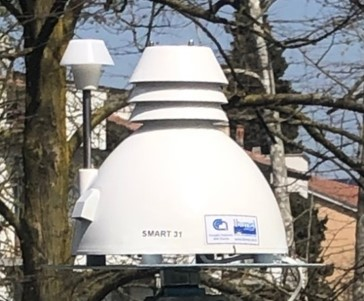
\includegraphics[width=.8\textwidth]{images/airqino_stazione}
\end{center}
\end{column}

\end{columns}
\end{frame}

\begin{frame}{La piattaforma AirQino (2/2)}
\end{frame}

%\section{Sviluppi tecnologici}
%
%
%\section{Calibrazione}
%
%
%\section{Interfaccia}
%
%
%\section{Conclusione}

